\documentclass{beamer}% {{{
\usepackage{amssymb, latexsym, amsmath, graphics, fullpage, epsfig, amsthm, relsize, pgf, tikz, amsfonts, makeidx, latexsym, ifthen, hyperref, calc}
%\usepackage{eucal} this is a different font than \mathcal{•}
\usetikzlibrary{arrows}
%\newtheorem{theorem}{Theorem}[section]
\newtheorem{remark}{Remark}[section]
%\newtheorem{corollary}{Corollary}
%\newtheorem{lemma}{Lemma}
\newtheorem{assumptions}{Assumptions}[section]
\newtheorem{proposition}{Proposition}
%\newtheorem{definition}{Definition}
\newtheorem{notation}{Notation}
\usepackage{mathrsfs}
%\usepackage[shortlabels]{enumitem}
\usepackage{tikz}
\usepackage{amsmath}
\usetikzlibrary{arrows}
\usetikzlibrary{shadows.blur}
\usepackage{pgfplots}
\usepackage{mwe} % For dummy images
\usepackage{subcaption}
\usepackage{multirow}
\usepackage{dcolumn}
\newcolumntype{2}{D{.}{}{2.0}}
\usepackage{multicol}
\numberwithin{equation}{section}

\newcommand{\lip}{\textup{Lip}_b}
\newcommand{\liph}{\text{Lip}_{\hat\rho}}
\newcommand{\R}{\mathbb{R}}
\newcommand{\E}{\mathbb{E}}
\newcommand{\Norm}[1]{\left\|  #1   \right\|}
\newcommand{\ud}{\ensuremath{\mathrm{d} }}

\newcommand{\mySeparateLine}{
	\begin{center}
		\makebox[\linewidth]{\rule{0.6\paperwidth}{0.4pt}}
\end{center}}
%\usepackage{lipsum}%% a garbage package you don't need except to create examples.
%\usepackage{fancyhdr}
%\pagestyle{fancy}
%\lhead{\Huge Version A}
%\rhead{\thepage}
%\cfoot{}
%\renewcommand{\headrulewidth}{0pt}



\setbeamersize{text margin left=2mm,text margin right=2mm}

\usepackage{animate}

\usepackage{tikz}
\usepackage{pgfplots}
\pgfplotsset{compat=newest}
\usetikzlibrary{decorations.markings}

\allowdisplaybreaks


\defbeamertemplate{footline}{higher page number}
{%
	\hfill%
	\usebeamercolor[fg]{page number in head/foot}%
	\usebeamerfont{page number in head/foot}%
	\insertframenumber\,/\,\inserttotalframenumber\kern1em\vskip20pt%
}
\setbeamertemplate{footline}[higher page number]

% }}}
% {{{ Title page
\title[About Beamer] %optional
{
Thesis Defense: \\ 
Invariant measures for the stochastic heat equation with no drift term
} 

\author[Arthur, Doe] % (optional, for multiple authors)
{Nicholas Eisenberg}


\date[VLC 2021] % (optional)
{ \small March 29, 2022 
}

\logo{\includegraphics[height=1cm]{overleaf-logo}}
\thispagestyle{empty}

\newcommand{\rdot}{\tikz\draw[red,fill=red] (0,0) circle (.5ex); \;}

\begin{document}
	\frame{\titlepage}	
	\setcounter{page}{1}

	\begin{frame}{The stochastic heat equation}
		\[
		\begin{cases}
		\dfrac{\partial u}{\partial t}(t,x)- \frac{1}{2}\Delta_xu(t,x) = b(x, u(t,x))\dot{W}(t,x), & t \ge 0, \: x \in \R^d
		\\ u(0,\cdot) = \mu(\cdot)  &
		\end{cases} \vspace{.1in}
		\]

\rdot The Stochastic Heat Equation is interpreted as follows: \vspace{0in}
\begin{align*}
u(t,x) &= \int_{\R^d} G(t,x-y) \mu(\ud y) + \int_0^t \int_{\R^d}G(t-s,x-y)b(u(s,y))W(\ud s, \ud y) 
\end{align*}
where $G(t,x)$ is the heat kernel \vspace{0in}
\[
G(t,x) = (2 \pi t)^{-d/2} \exp\left(- \frac{|x|^2}{2t} \right) \vspace{.1in}
\]
\rdot A processes, $\{u(t,x) : t \ge 0, \; x\in \R^d \}$, that satisfies this relation is referred to as the {\it mild solution}.


\end{frame}

\begin{frame}[t]{The noise term $\dot{W}$}
\rdot $W = \{W(\phi): \: \phi \in \mathscr{S}(\R^d) \}$ is a centered Gaussian process uniquely defined through the following covariance functional: 
\[
	J(\phi, \psi) := \mathbb{E}\left[W(\phi)W(\psi)\right] = \int_0^\infty \ud s \int_{\R^d} \Gamma(\ud x) (\phi(s,\cdot)*\tilde{\psi}(s,\cdot))(x),
\]
where $\tilde{\psi}(s,x) = \psi(s,-x)$. We have the following nomenclature. \vspace{.25in} 
	
 \rdot {\em Space-time white noise}: $\Gamma(\ud x) = \delta_0(\ud x)$. \vspace{.15 in}
 
 \rdot {\em Time white and spatially colored:} $\Gamma(\ud x) = f(x)\ud x$ where $f$ is a non-negative and non-negative definite function referred to as the {\em Correlation function} and its Fourier transform,
 	\[
 		\widehat{f}(\xi) := \mathcal{F}f(\xi) = \int_{\R^d} \exp\left(-i x \cdot \xi\right) f(x) \ud x,
 	\]
 is referred to as the {\em spectral density}.
\end{frame}

\begin{frame}[t]
	\begin{proposition}[DaPrato and Zabczyk {\cite[Propsition 4.19]{DZ19}}]
		A space-time white noise is the distributional derivative of a Brownian sheet, $B(t,x)$.
	\end{proposition}

\begin{figure}[t]
	\centering
	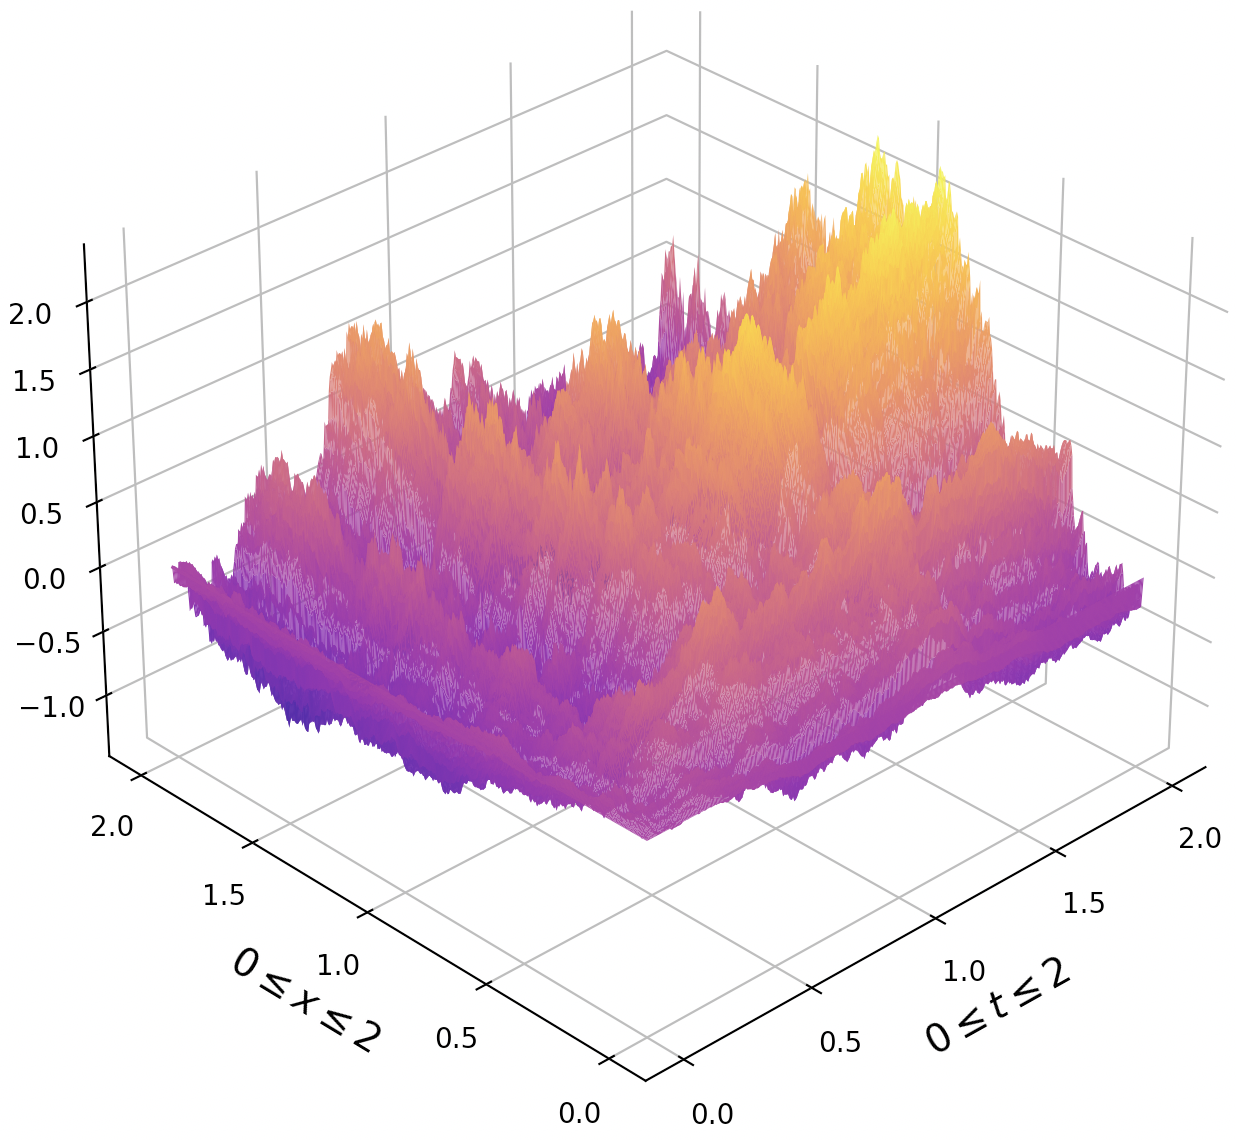
\includegraphics[scale=.28]{figs/bsheet.png}
	\caption{Brownian Sheet Simulation (Walsh \cite{Walsh}): \\
		$B(t,x) \sim B(t - \delta_t, x) + B(t, x- \delta_x) - B(t - \delta_t, x - \delta_x) + \text{normal}(0, \delta_t \delta_x)$ \\
		$B(t,0) = B(0,x) = 0$ for all $t,x >0$.
	}
\end{figure}
\end{frame}

\begin{frame}{Existence and uniqueness with space-time white noise}
	\rdot A necessary condition for global existence, {\em Dalang's condition} \cite{Dal99}, is the following:
	\[
		\int_0^t \ud s \int_{\R^d} \ud y \: G^2(s,y) < \infty, \quad \forall t > 0.
	\] 
	\rdot Direct calculation yields that,
	\[
		\int_0^t \ud s \int_{\R^d} \ud y \: G^2(s,y) = 
		\frac{\Gamma(d/2)}{2(2\pi)^d} \int_0^t \frac{1}{s^{d/2}} \ud s,
	\]
	which forces,
	\[
		d/2 < 1 \quad \iff \quad d < 2.
	\]
	\rdot Thus a global space-time white noise solution may only exist when the spatial dimension is $1$. 
\end{frame}

\begin{frame}{Large Peaks: $u_t - \frac{1}{2}u_{xx} = \lambda u \dot{W}$ with $u_0(x) = \delta_0(x)$ \\ driven by a space-time white noise}
	\begin{center}
		$\lambda = 0$ 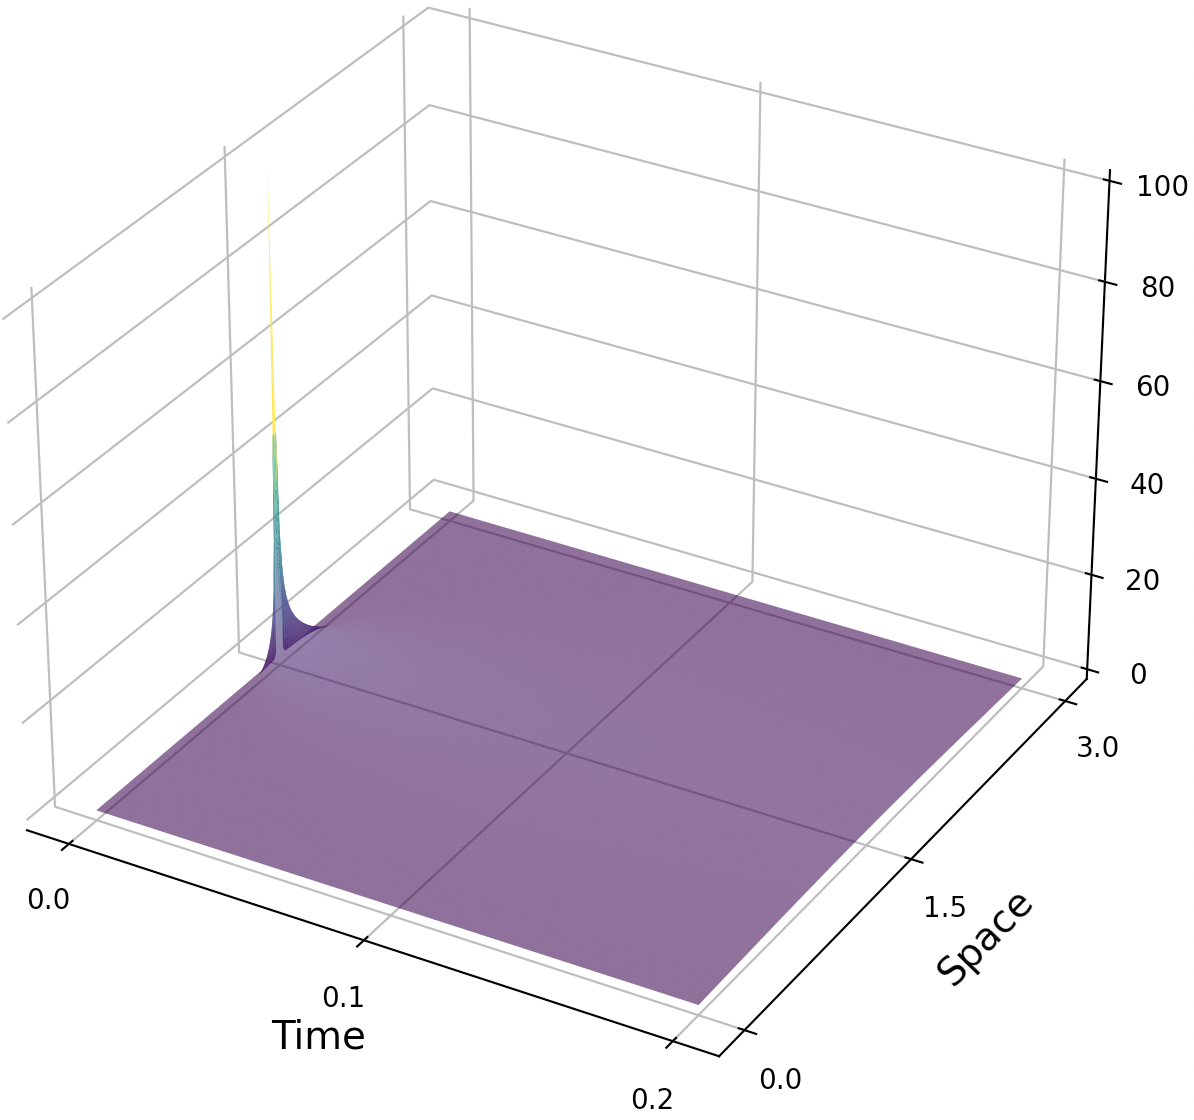
\includegraphics[scale=.2]{figs/SHE0.png} \quad  $\lambda = 1$ 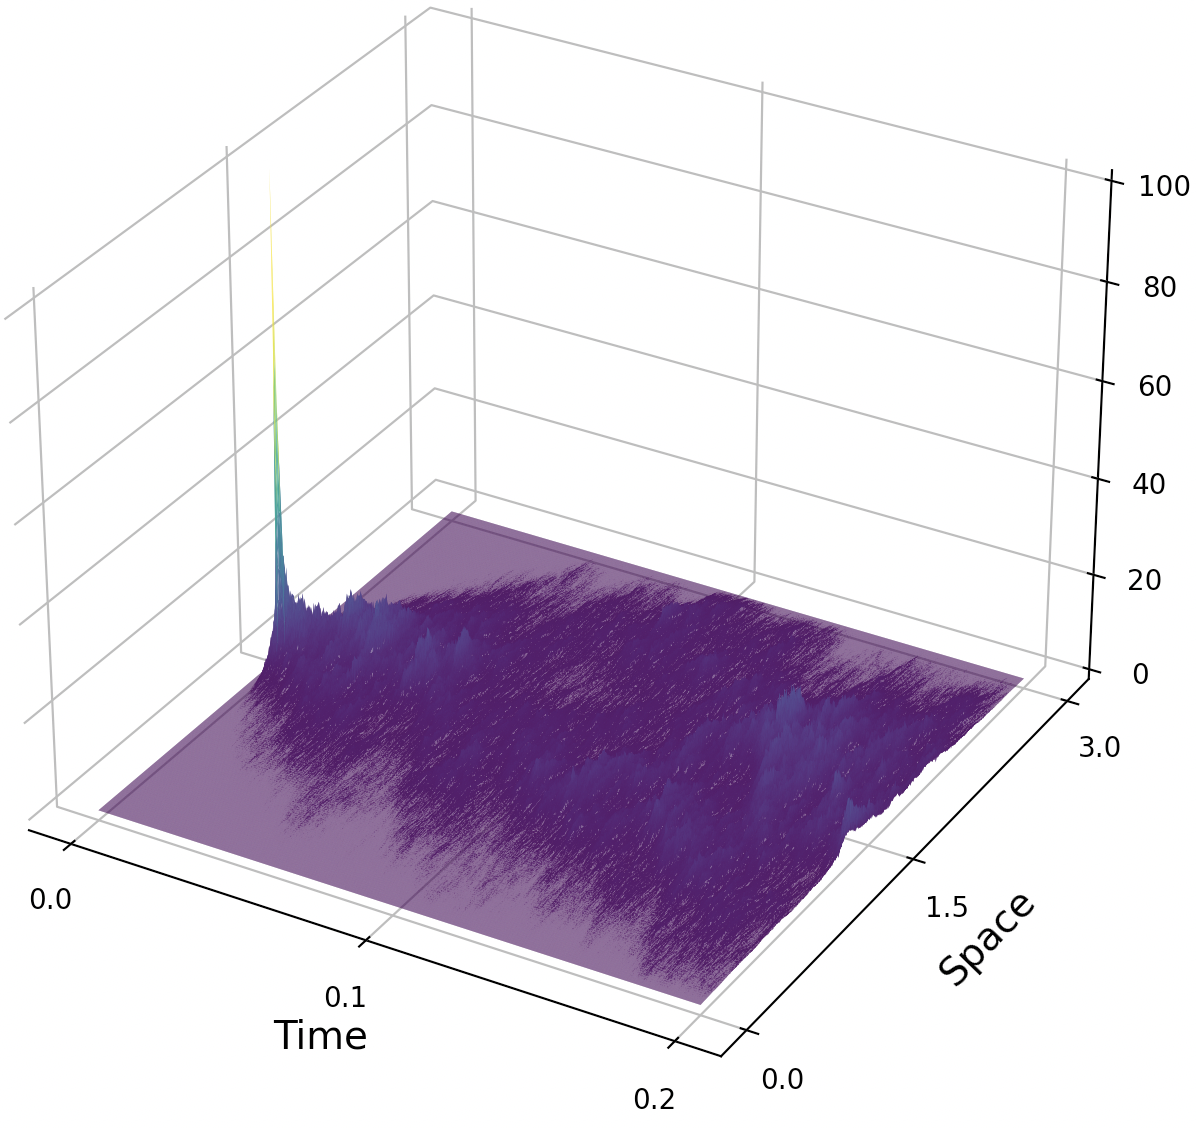
\includegraphics[scale=.2]{figs/SHE1.png}
	\end{center}
\rdot Simulations done by using a finite difference scheme \cite{DG2000}. \\
\rdot We partition (space) $[0,3]$ into $n_x$ pieces of size $\delta_x = 3 / n_x$. \\
\rdot We partition (time) $[0, .2]$ into $n_t$ pieces of size $\delta_t = .2 / n_t$.
	\begin{align*}
		u(t+\delta_t, x) &= u(t,x) + n_x^2 \delta_t \left( u(t, x + \delta_x) + u(t, x - \delta_x) -2 u(t,x) \right)  \\
		& \qquad \quad + n_x \lambda u(t,x) \: \text{normal}(0, \delta_t \delta_x).
	\end{align*}
\end{frame}

\begin{frame}{Intermittency of $u_t - \frac{1}{2}u_{xx} = \lambda u \dot{W}$ driven by space-time white noise}
	\begin{center}
		$\lambda = 1.8$ 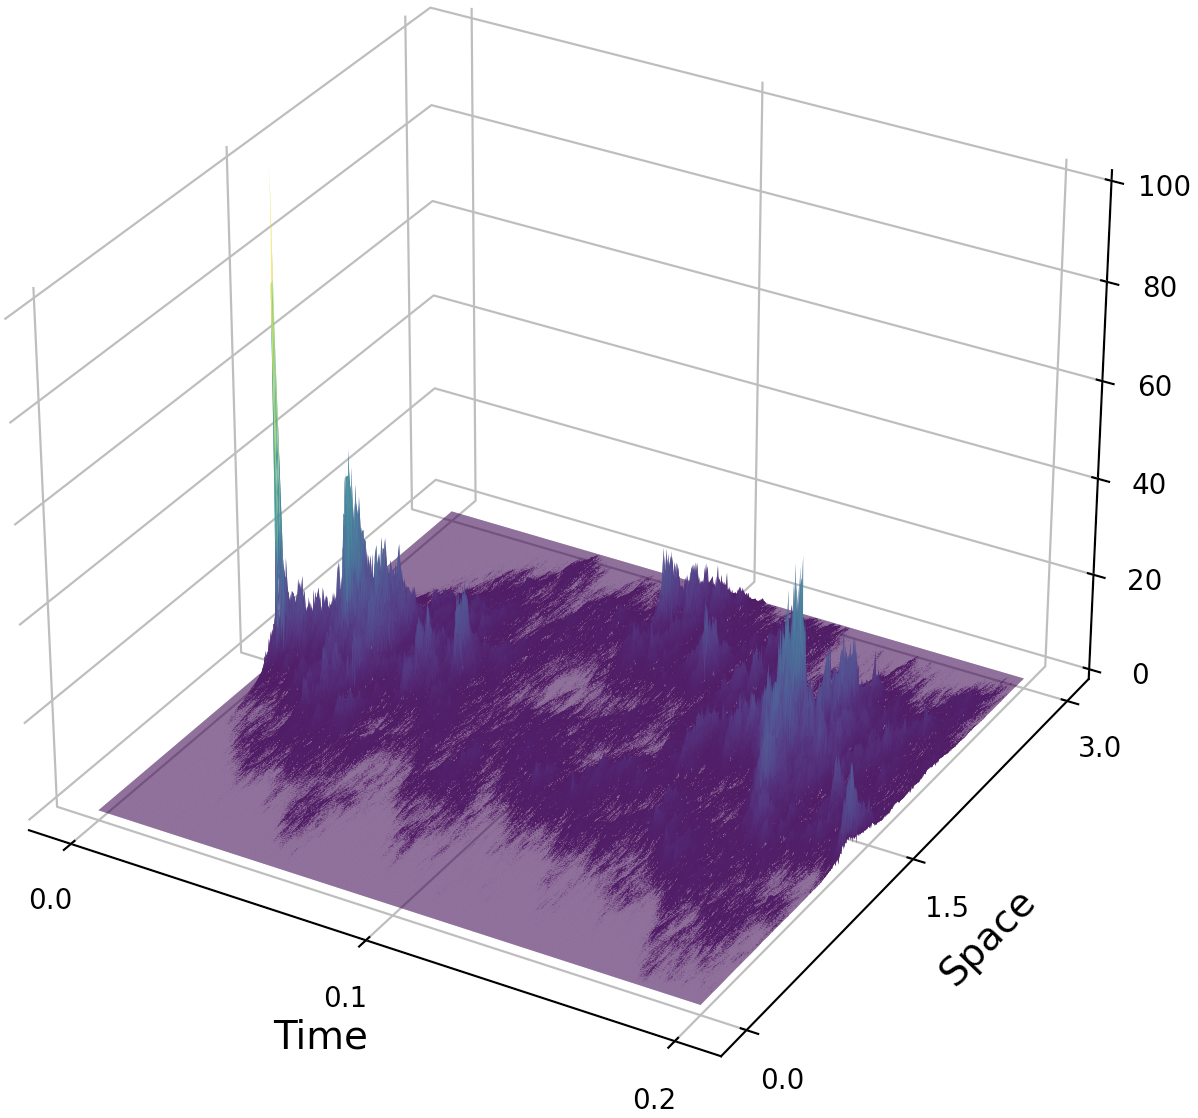
\includegraphics[scale=.2]{figs/SHE1.8.png} \quad $\lambda = 2$ 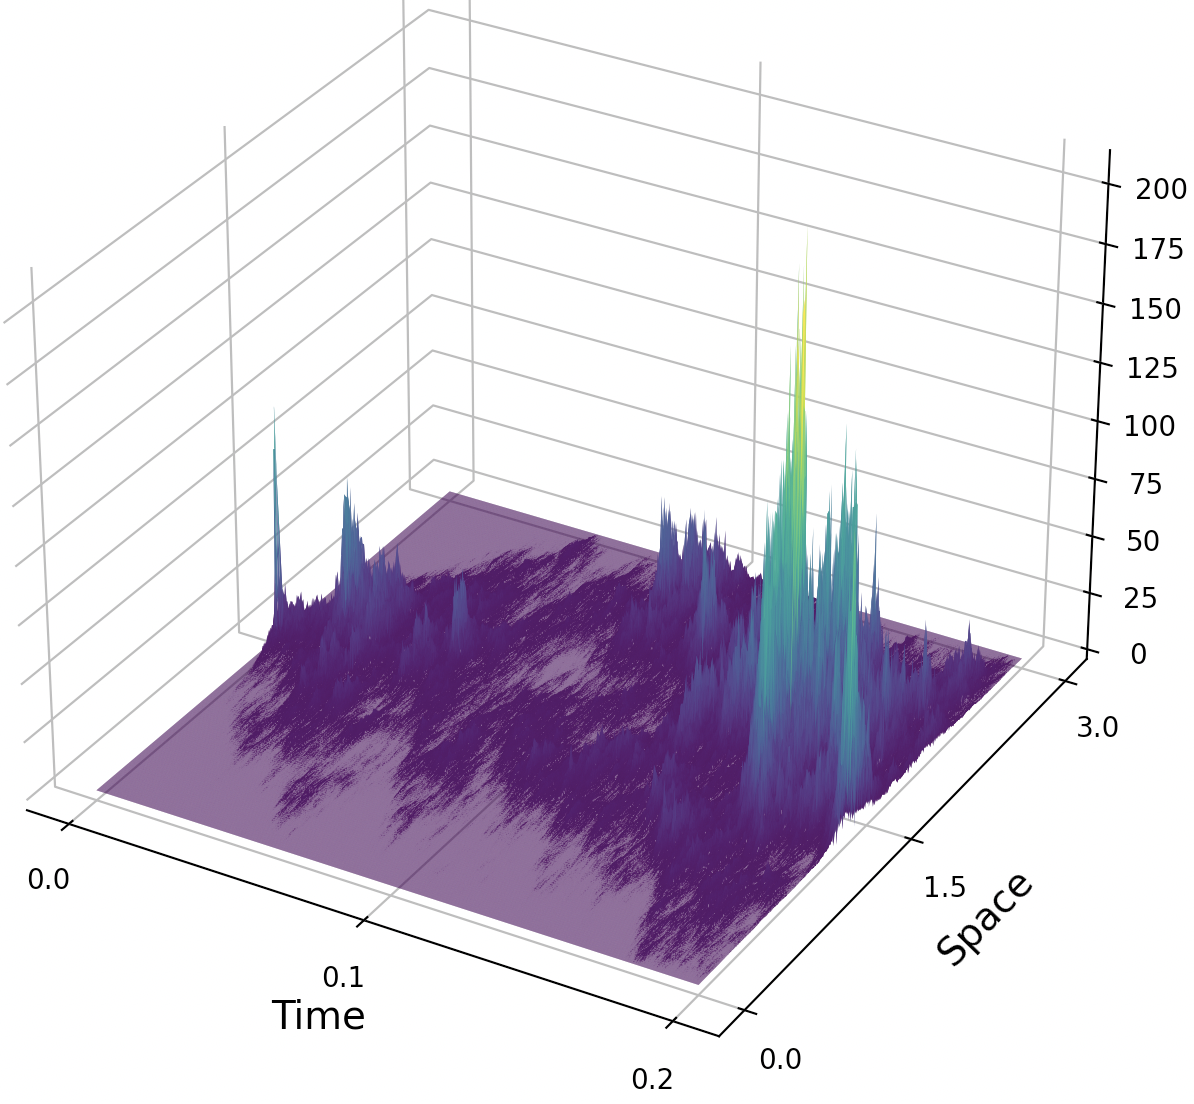
\includegraphics[scale=.2]{figs/SHE2.png}
	\end{center}
\rdot Notice the enlargement of the peaks as $\lambda$ increases. We have the following theorem. \vspace{.1in}
\begin{theorem}[Chen and Dalang {\cite[Theorem 2.4]{CD15}}]
	The second moments of the stochastic heat equation driven by space-time white noise grow exponentially in time. 
\end{theorem}
\end{frame}

\begin{frame}{Will the second moments ever be bounded in time?}
	\rdot Several slides below will require the second moments to be bounded in time:
		\[
			\sup_{t\ge0} \Norm{u(t,x)}_2 < \infty, \qquad \text{where } \Norm{X}_p = \left[\mathbb{E}\left(|X|^p\right)\right]^{1/p}.
		\]
	
	\rdot This is possible, however this will require us to only consider $d \ge 3$, and therefore we must only consider a spatially colored noise. \vspace{.2in}
	
	\rdot Recall from above, that the covariance of a spatially colored noise is given by the following:
	\begin{align*}
 \mathbb{E}\left[W(\phi)W(\psi)\right] &= \int_0^\infty \ud s \int_{\R^d} \ud x \: f(x) (\phi(s,\cdot)*\tilde{\psi}(s,\cdot))(x) \\
 &= \int_0^\infty \ud s \int_{\R^{2d}} \ud x \ud y \: \phi(s,x)f(x-y)\psi(s,y) \\
 &= (2\pi)^{-d} \int_0^{\infty} \ud s \int_{\R^d} \ud \xi \: \widehat{f}(\xi) \mathcal{F}\phi(s,\xi) \overline{\mathcal{F}\psi(s,\xi)}
 \end{align*}
\end{frame}
	
\begin{frame}{Existence and Uniqueness with a Colored Noise}
\begin{theorem}[Chen and Huang {\cite[Theorem 1.2]{CH19}}]
There exists a unique global mild solution under the following:
\end{theorem} \vspace{.1in}

\rdot $b: \R^d \times \R \to \R$ such that there exists a $L_b,L_0 >0$ so for all $u,v \in \R$ and $x \in \R^d$,
\[
|b(x,u)-b(x,v)| \le L_b|u-v| \quad \text{and} \quad  |b(x,0)| \le L_0.
\] \vspace{0in}

\rdot The initial measure, $\mu(\ud x)$ (resp. $\varphi(x) \ud x$), satisfies for some $a > 0$,
\[
\int_{\R^d} e^{-a|x|^2} |\mu|(\ud x) < \infty \quad \left(\text{resp. } \int_{\R^d} e^{-a|x|^2} |\varphi(x)|\ud x < \infty \right),
\] 
where $|\mu| = \mu^+ + \mu^-$ is the {\em Hahn decomposition}. \vspace{.2in}

\rdot The spectral density,$\widehat{f}$, satisfies {\it Dalang's condition for some $\beta >0$:}
\[
\Upsilon(\beta) : = \int_{\R^d} \frac{\hat{f}(\ud \xi)}{\beta + |\xi|^2} < \infty.
\]

\end{frame}

		\begin{frame}
	\frametitle{References}
	\small
	
	\begin{thebibliography}{999}
		\bibitem{CD15}
		L. Chen and R. Dalang (2015)
		\newblock{Moments and growth indices for the nonlinear stochastic heat equation with rough initial conditions} 
		\newblock {\em The Annals of Probability} 43, 6, 3006--3051
		
		\bibitem{CH19} 
		L. Chen and J. Huang
		\newblock Comparison principle for stochastic heat equation on $\R^d$
		\newblock {\em  Ann. Probab}, 47.2 (2019) 989--1035.
		
		\bibitem{CHN19} 
		L. Chen, Y. Hu, D. Naulart (2019)
		\newblock Nonlinear stochastic time-fractional slow and fast diffusion equations on $\R^d$.
		\newblock {\em  Stochastic Processes and their Applications}, 129 5073--5112.
		
		\bibitem{CK19}
		L. Chen and K. Kim (2019)
		\newblock Nonlinear stochastic heat equation driven by a spatially colored noise: moments and intermittency.
		\newblock {\em Acta Mathematica Scientia} 39B(3), 645--668
		
		\bibitem{DG2000}
		A. Davie and J. Gaines (2000)
		\newblock Convergence of numerical schemes for the solution of parabolic stochastic partial differential equations
		\newblock{\em Mathematics of Computation} 70, 223, 121---134
		
		\bibitem{Dal99}
		R. Dalang (1999)
		\newblock Extending the martingale measure stochastic integral with applications to spatially homogeneous s.p.d.e.'s
		\newblock {\em  Electron. J. Probab.}
		
		\bibitem{DZ19}
		G. DaPrato and J. Zabczyk (2014)
		\newblock Stochastic Equations in Infinite Dimensions. 2nd Edition.
		\newblock {\em  Cambridge University Press}
		
		\bibitem{Walsh}
		J. Walsh (1986)
		\newblock Introduction to Stochastic Partial Differential Equations
	\end{thebibliography}
\end{frame}

\end{document}
